\documentclass[conference]{IEEEtran}

\usepackage[utf8]{inputenc}
\usepackage{cite}
\usepackage{amsmath}
\usepackage{graphicx}
\usepackage[english,hungarian]{babel}
\usepackage[section]{placeins}
    
\begin{document}
\selectlanguage{english}

\title{Image Inpainting for Regular Holes Using Partial Convolutions\\
	{\large \textbf{Szabályos lyukak digitális retusálása részleges konvolúcióval}}\\
	{\large \textit{Team:} DeepPurple}\\
}

\author{
	\IEEEauthorblockN{Dávid Kékesi}
	\IEEEauthorblockA{
		J9PCWO \\
		david.kekesi@gmail.com}
\and
	\IEEEauthorblockN{Mátyás Sándor}
	\IEEEauthorblockA{
		YHMJTY\\
		sandor.matya@t-online.hu}
\and
	\IEEEauthorblockN{Zoltán Király}
	\IEEEauthorblockA{
		G24TCR\\
		ze.kiraly@gmail.com}
}

\maketitle

\selectlanguage{english}
\begin{abstract}\\
Image inpainting is the process of restorating a missing, undesired or damaged part of an image.
Initially, the technical faults of early cameras (scratches, stains) were corrected by experts while the development of photos. 
Although nowadays the manipulation of images happens digitally, the proper way of inpainting still requires skilled hands.
Many effort have been made to solve the automatization of this method. In this paper, we represent our work on applying
a model based on partial convolutions to fill missing parts of images with natural looking content.
\end{abstract}

\selectlanguage{hungarian}
\begin{abstract}\\
A folyamatot, melynek során egy kép sérült, nem kívánatos vagy hiányzó részeit eltüntetjük, retusálásnak nevezzük.
A fényképezőgépek technikai hibáit (karcok, pöttyök) eleinte manuálisan küszöbölték ki a szakemberek a fotók előhívás során.
Bár a fényképek manipulációja napjainkban digitális úton történik, a megfelelő retusálás továbbra is hozzáértő kezeket igényel.
A művelet automatizálására számos megoldás létezik, Jelen munkában azt mutatjuk be, hogy hogyan alkalmaztunk egy
részleges konvolúcióra épülő modellt, mely képes képek hiányzó részeit kiegészíteni természetes hatású tartalommal.
\end{abstract}

\selectlanguage{english}
\begin{IEEEkeywords}
Deep Learning, neural network, Image inpainting, GAN
\end{IEEEkeywords}

\section{Introduction}
At the initial stage of the project the team had consensus that we would like to work on a project involved in image processing. In the field of image inpainting Nvidia’s 2018 solution based on partial convolutions was a huge step forward, so this fileld seemed to be exciting enough to start working on. All of the team members are perfectly new to the filed of deep learning, so we had to start with lots of reading and information gathering. Fundamentallyit seemed that there are two widely used approahches for restoring the missing parts of an image. The first one is using a GAN, where a VAE based generator network, and a discriminator network, competing each other, creates more and more realistic images in a given domain. With a bit of modification this approach can be used not only for generating images from scratch, but for filling in the missing parts of an image as well. The other approach was based on the paper of Liu \cite{nvidia_paper}. It was obvious that both approaches require a lot of time spent on training, and we had limited hardware resources. The GAN approach had a further drawback: it’s very hardto do it in a way that it really gives usable results, and the network needs a lot of fine tuning. Reading the above linked paper, we found out that implementing the partial convolution can lead us to a shortcut, where we can use transfer learning by reusing the alredy trained VGG\_16 network, saving usa reasonable amount of GPU time. Even so the adaptation of the paper was quite difficult for us, being total beginners, so our final solution relies heavily on a Keras adaptation that we found on GitHub \cite{pconv_keras}. Even with the use of transfer learning we had to train the adapted model for 7-8 hours per training (60-70 epochs) on a GTX 1060, but the final results are quite impressive on the choosen dataset

\section{Data acquisition and preparation}
We used the Caltech-UCSD Birds-200-2011 dataset \cite{dataset}. It consists of 11788 annotated photos of 200 different bird species.

As preparation, we calculated the minimal bounding square of birds according to their bounding boxes. Through this process, we threw away the images where the bounding box couldn't be contained in a square due to the original image dimensions. We then translated the resulting square to a resolution of 256  $\times$ 256 pixels.

This way we got 9581 images which we splitted into train, validation and test sets in a 6:2:2 ratio. 

For the training, we use a 64 $\times$ 64 pixel hole in the center of the image.

\begin{figure}
  \centering
  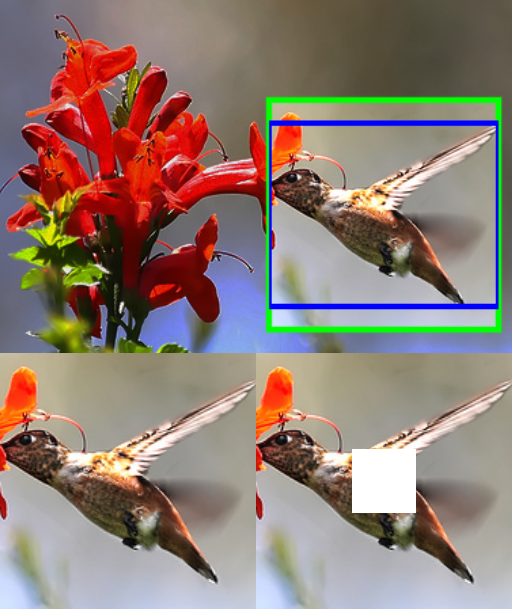
\includegraphics[width=80mm, keepaspectratio]{figures/preparation.png}
  \caption{The original image with bounding box (red) and the minimal square (green) and the resulting image with the applied mask}
  \label{fig:Preparation}
\end{figure}


\section{Initial method}
There are two main components ofthe learning process in the chosenproblem: an encoder an adiscriminator network has to workagainst each other, in order tomotivate each other to produce betterand better outputs, thus eliminatingthe differences bethween the originaland generated pictures, and, ont hediscriminator side to learn the  smallerand smaller differences bethween thegenerated and real pictures, thusmotivating the encoder to eliminatethe said smaller and smallerdifferences as well. 

\begin{figure}
  \centering
  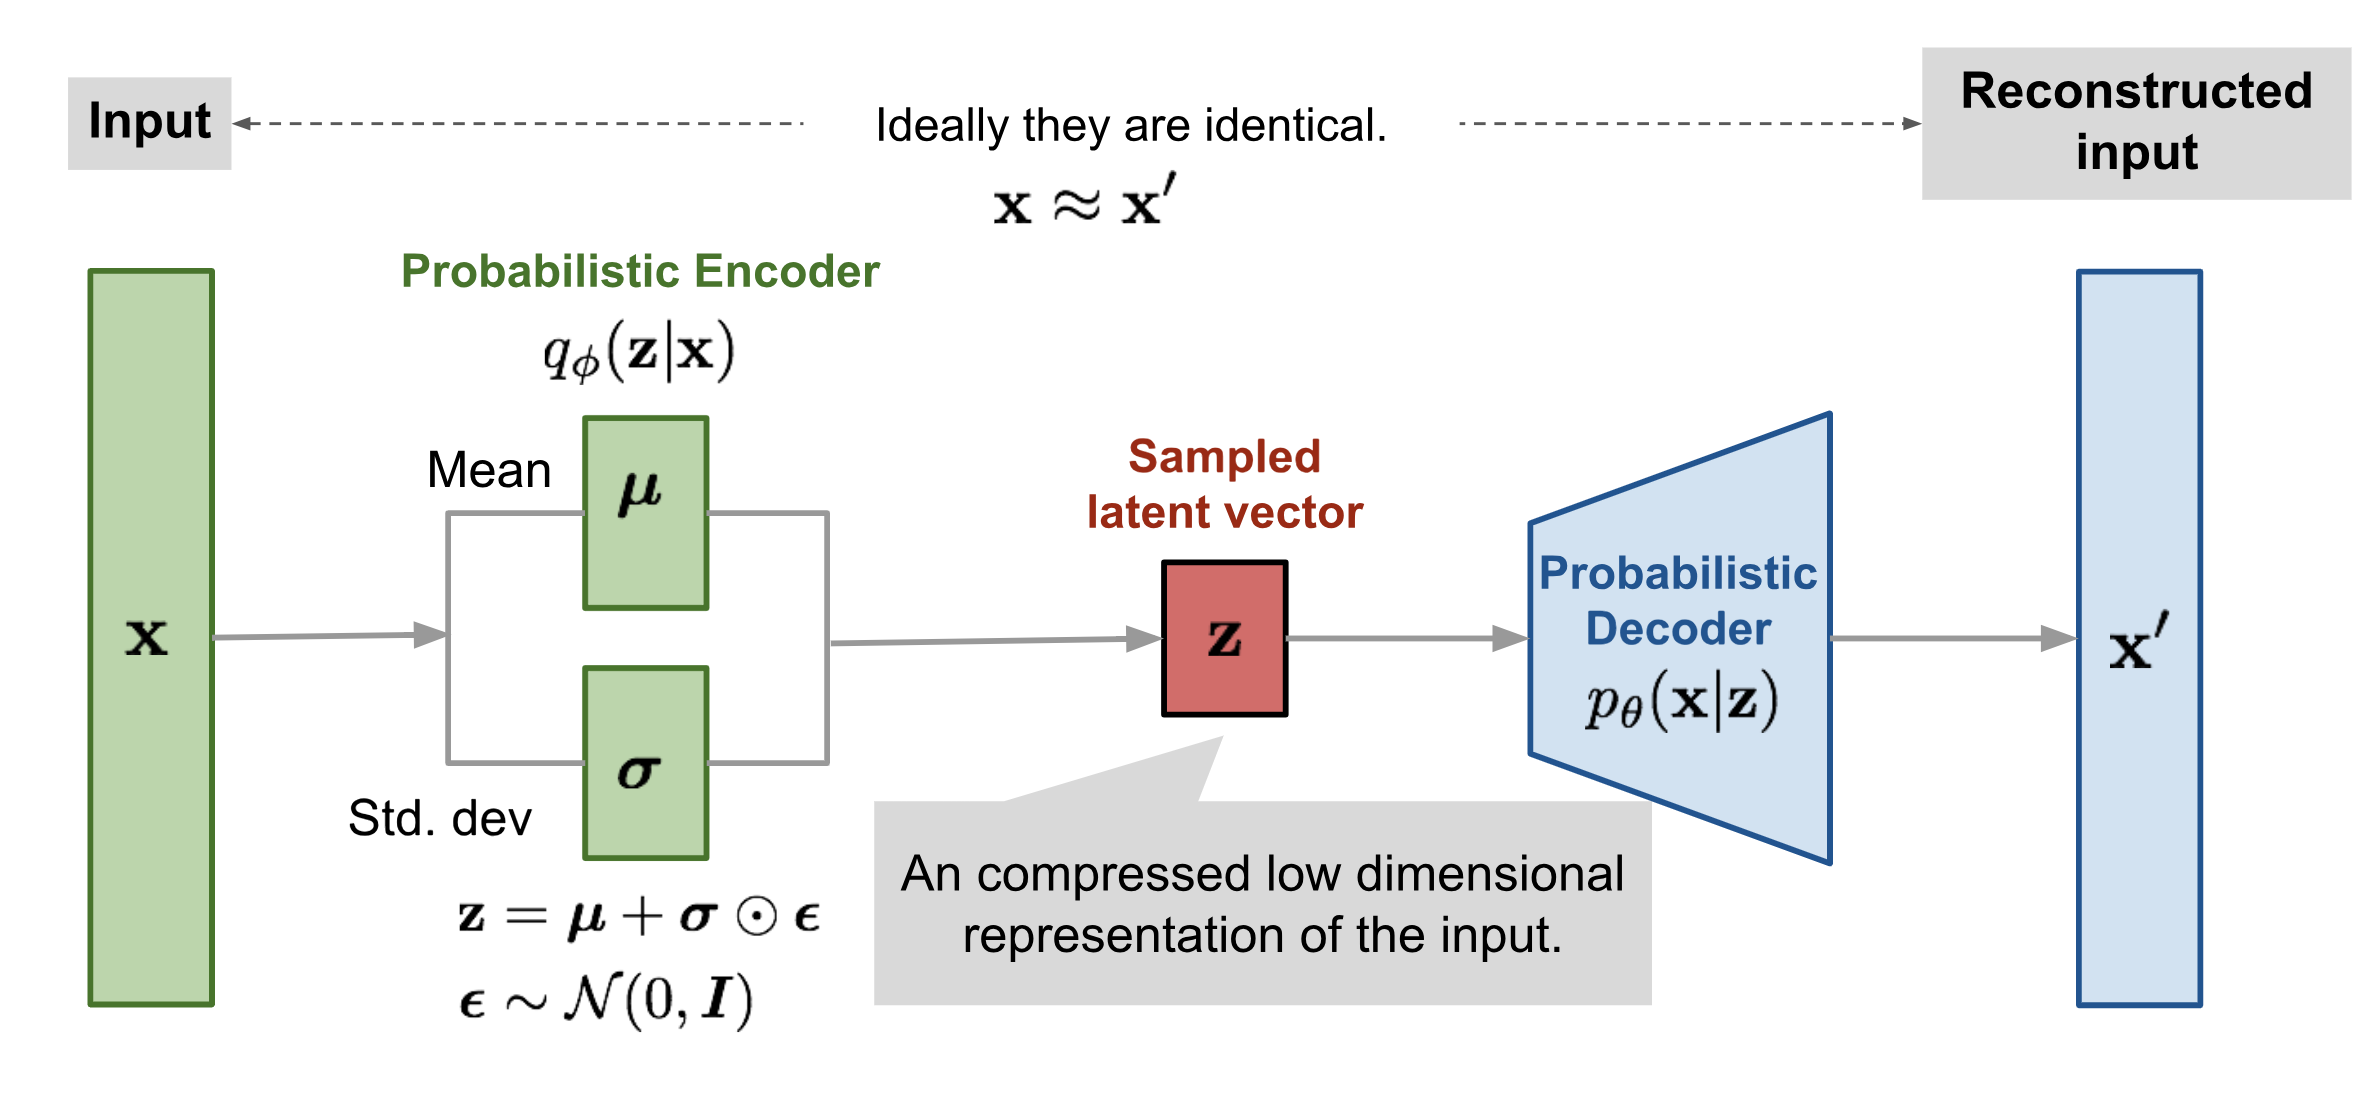
\includegraphics[width=80mm, keepaspectratio]{figures/vae-gaussian.png}
\end{figure}

\begin{figure}
  \centering
  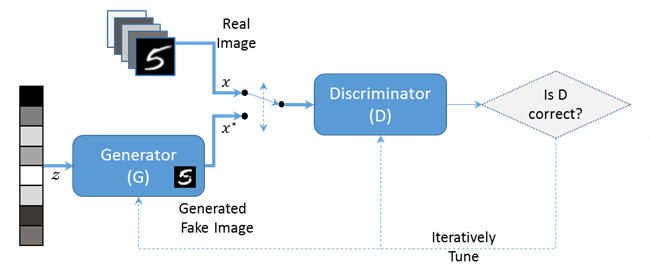
\includegraphics[width=80mm, keepaspectratio]{figures/GAN_basic_flow.png}
\end{figure}

We tried to use the above described method to solve the given problem, but before implementing the intially found method as a solution, we found a more modern approach, one that was more promising, and indeed proved to be a viable and fuitful solution.

\section{Partial convolution}
The applied network relies on the use of a layer consisting of partial convolution and automatic mask update.
The partial convolution can be defined as
\begin{equation}
{x}' = \begin{cases}
W^T(X \odot M) \frac{sum(1)}{sum(M)} + b, & \text{if } sum(M) > 0 \\
0, & \text{otherwise}
\end{cases}
\end{equation}
for every location, where W is the weight matrix for the convolution filter and b is its corresponding bias. X are the feature values for the current convolution window and M is the curresponding binary mask.
$\odot$ denotes element-wise multiplication, and 1 has the same shape as M but with all elements being 1. Output values depend only on the unmasked inputs. The scaling factor sum(1)/sum(M) applies appropriate scaling for the varying amount of valid (unmasked) inputs.

After each partial convolution operation, we then update our mask as follows:
if the convolution was able to condition its output on at least one valid input value, then we mark that location as valid. This is expressed as:

\begin{equation}
{m}' = \begin{cases}
1, & \text{if } sum(M) > 0 \\
0, & \text{otherwise}
\end{cases}
\end{equation}

And can be implemented in any deep learning framewrok as part of the forward pass. With sufficient successive applications of the partial convolution layer, any mask will eventually be all ones, if the input contained any valid pixels.

\section{Partial Convolution as Padding}
We use the partial convolution with
appropriate masking at image boundaries in lieu of typical padding . This ensures
that the inpainted content at the image border will not be affected by invalid
values outside of the image – which can be interpreted as another hole.

\section{Partial Convolution Substituting Convolution}
Before using partial convolution, it was widely accepted, that regular convolution networks arethe best suited for image imprinting, When usingregular convolution networks, the image oftenbecomes blurried, the color sclae shifts, or theresulting image is not acceptabe for otherreasons:e.g. the outlines of the cutout show. A few visual examples are shown below.

\begin{figure}[!htb]
  \centering
  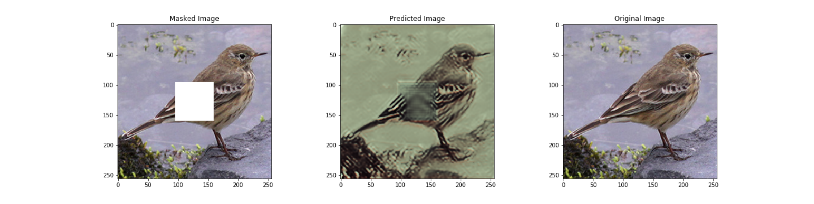
\includegraphics[width=80mm, keepaspectratio]{figures/err_1.png}
\end{figure}

\begin{figure}[!htb]
  \centering
  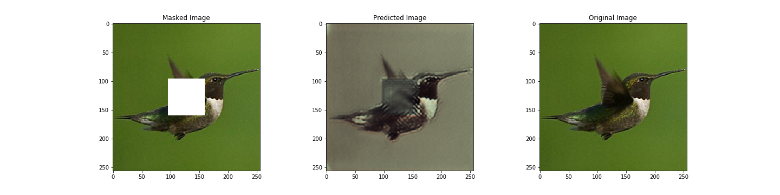
\includegraphics[width=80mm, keepaspectratio]{figures/err_2.png}
\end{figure}

\begin{figure}[!htb]
  \centering
  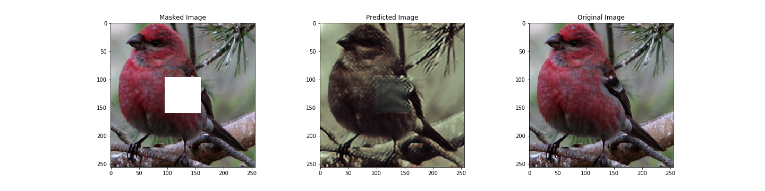
\includegraphics[width=80mm, keepaspectratio]{figures/err_3.png}
\end{figure}

These pictures are the results of previous trainings 
The old solution to the afformentioned problem was post-processing, which was a computationally expensive process, as well as an unreliable one, as it often failed.
Partial convolutions are a relatively newly introduced solution to the image inprinting problem 

\section{Results}

\begin{figure}[!htb]
  \centering
  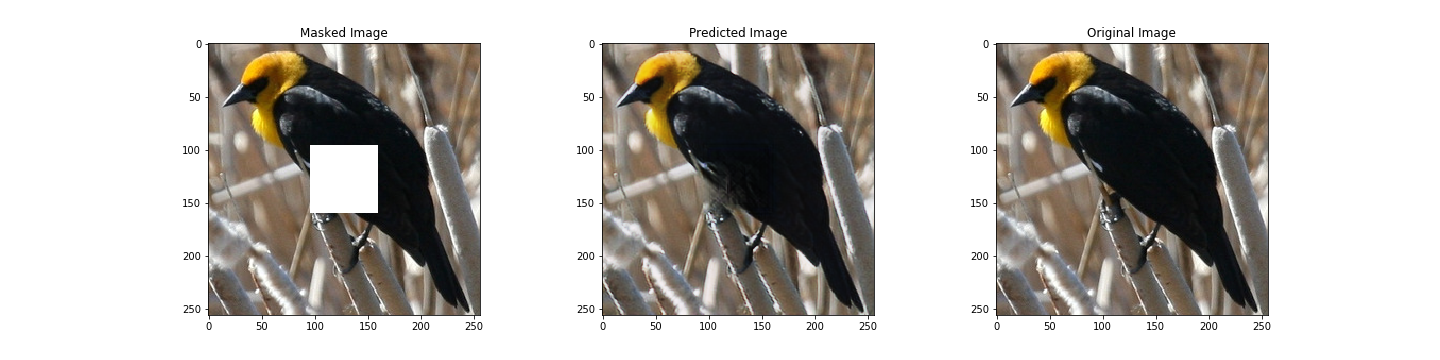
\includegraphics[width=80mm, keepaspectratio]{figures/result_1.png}
\end{figure}

\begin{figure}[!htb]
  \centering
  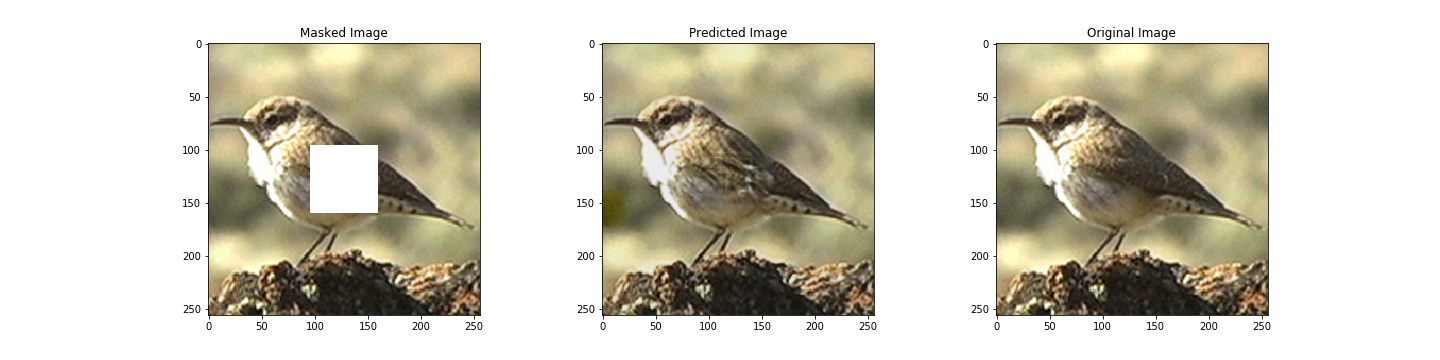
\includegraphics[width=80mm, keepaspectratio]{figures/result_2.png}
\end{figure}

\begin{figure}[!htb]
  \centering
  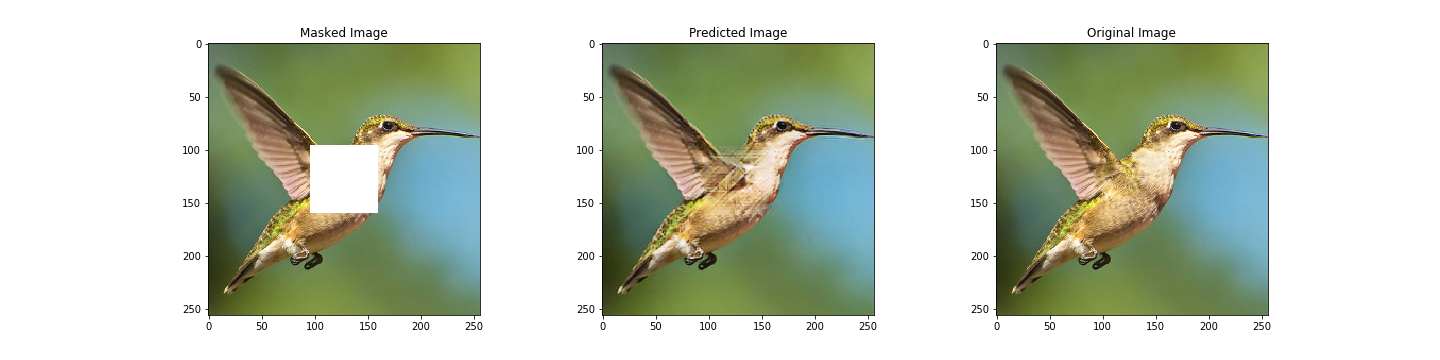
\includegraphics[width=80mm, keepaspectratio]{figures/result_3.png}
\end{figure}

\begin{figure}[!htb]
  \centering
  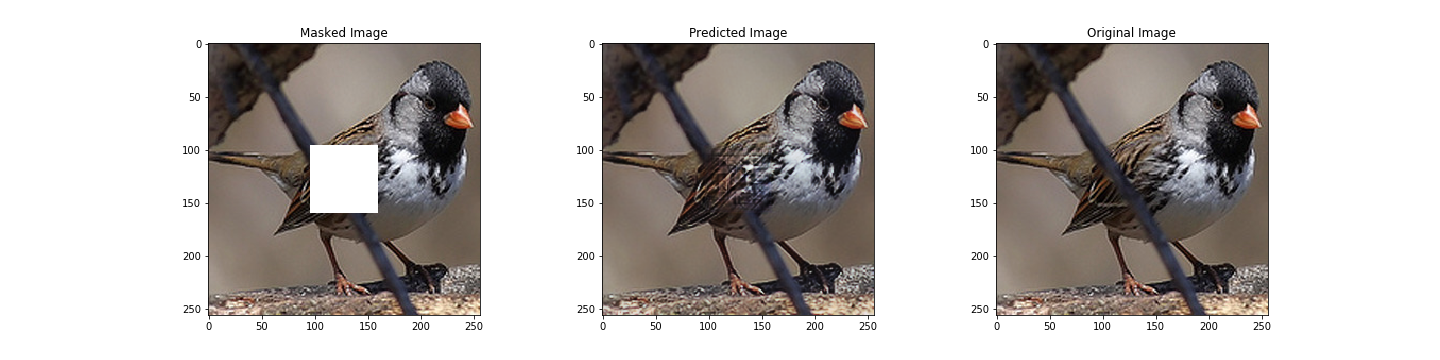
\includegraphics[width=80mm, keepaspectratio]{figures/result_4.png}
\end{figure}

\begin{figure}[!htb]
  \centering
  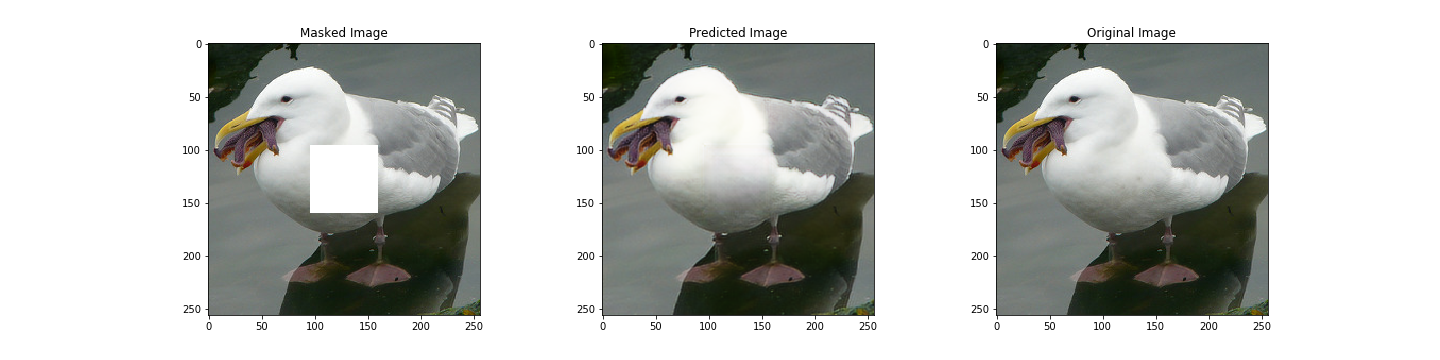
\includegraphics[width=80mm, keepaspectratio]{figures/result_5.png}
\end{figure}

As you can see in the pictures, the results are mixed. Generally speaking, the network was able to fill out the pictures, and it added relevant details, completed feather patterns and limbs. However, in unusual situations, such as fast moving birds or birds with part of them hidden behind objects,  the neural network was unable to correctly guess the original image. 
The reason behind this is most likely due to the scarce nature of such photographs in the training database. Which is to be expected. 
However, all things considered the results are more than acceptable, and exceeded our expectations in situations where the feather pattern was recognisable, and in a few places even in difficult situations. (e.g: the 2nd picture, where the lighting is really difficult, and the feather pattern is mostly hidden as well.)

\vspace{20px}
\begin{thebibliography}{00}

\bibitem{dataset} Wah, C. and Branson, S. and Welinder, P. and Perona, P. and Belongie, S., ``The Caltech-UCSD Birds-200-2011 Dataset'', California Institute of Technology, CNS-TR-2011-001, 2011

\bibitem{nvidia_paper} Guilin Liu, Fitsum A. Reda, Kevin J. Shih, Ting-Chun Wang, Andrew Tao, Bryan Catanzaro, ``Image Inpainting for Irregular Holes Using Partial Convolutions'', arXiv:1804.07723v2  

\bibitem{pconv_keras} https://github.com/MathiasGruber/PConv-Keras/

\bibitem{} Bertalmio, M., Sapiro, G., Caselles, V., Ballester, C., ``Image inpainting. In: Proceedings of the 27th annual conference on Computer graphics and interactive techniques'', pp. 417–424. ACM Press/Addison-Wesley Publishing Co. (2000)  

\bibitem{} Jiahui Yu, Zhe Lin, Jimei Yang, Xiaohui Shen, Xin Lu, Thomas S. Huang, ``Generative Image Inpainting With Contextual Attention. In: IEEE Conference on Computer Vision and Pattern Recognition (CVPR)'', pp. 5505-5514, 2018

\bibitem{} Dai, J., Qi, H., Xiong, Y., Li, Y., Zhang, G., Hu, H., Wei, Y., ``Deformable convolutional networks'', CoRR, abs/1703.06211 1(2), 3, 2017

\bibitem{} Harley, A.W., Derpanis, K.G., Kokkinos, I., ``Segmentation-aware convolutional networks using local attention masks'', In: IEEE International Conference on Computer Vision (ICCV). vol. 2, p. 7, 2017

\bibitem{} He, K., Zhang, X., Ren, S., Sun, J., ``Delving deep into rectifiers: Surpassing humanlevel performance on imagenet classification'', In: Proceedings of the IEEE international conference on computer vision. pp. 1026–1034, 2015


\end{thebibliography}

\end{document}